\subsection{I2S decoder and encoder}
The ADC and DAC use I2S to transfer the sampled audio data to the FPGA. This protocol needs to be decoded to obtain the actual data, processed and be encoded again to I2S to send to the DAC. The VHDL code that has been written for this can be found in \nameref{chap:appendix-B-vhdl}. 

\subsection{I2C controller}
The DAC must be configured with I2C. To be able to do this an I2C master must be programmed in the FPGA. This I2C master initializes the DAC with default configurations. The VHDL code of the I2C master can be found in \nameref{chap:appendix-B-vhdl}. 

\subsection{Band-pass filter}
In order to successfully compute the state-space band-pass filter output, the discrete state-space coefficients are needed. The equations for the discrete coefficients are seen in equation \ref{eq:discrete-coef-Ad} and equation \ref{eq:discrete-coef-Bd}.

\begin{equation}
    Ad=e^{AT}
    \label{eq:discrete-coef-Ad}
\end{equation}

\begin{equation}
    Bd=\frac{Ad-I}{A}\cdot B
    \label{eq:discrete-coef-Bd}
\end{equation}

Because the coefficients are all matrices, doing an exponent computation is a very expensive task for an FPGA. Therefore the exponent is rewritten with the taylor series to obtain equation \ref{eq:taylor-series-Ad} and equation \ref{eq:taylor-series-Bd}. The higher the value of n in the sum for Ad and Bd the less of an effect that new value has on the sum. Therefore having the sum go from $n=0\ to\ n=10$ is more than enough for the coefficients to be almost exact. The coefficients need to be computed only at the startup of the firmware and when the parameters of the band-pass filter change. 

\begin{equation}
    Ad=\sum_{n=0}^{\infty}\frac{A^n\cdot T^n}{n!}
    \label{eq:taylor-series-Ad}
\end{equation}

\begin{equation}
    Bd=\sum_{n=1}^{\infty}\frac{A^{n-1}\cdot T^n}{n!}\cdot B
    \label{eq:taylor-series-Bd}
\end{equation}

When every sample is being loaded into the state-space band-pass filter effect, the new state variables and the output will be computed according to equation \ref{eq:state-state-equation} and equation \ref{eq:state-output-equation}. 

\begin{equation}
    \dot{x}=Ad \cdot x + Bd \cdot u
    \label{eq:state-state-equation}
\end{equation}

\begin{equation}
    y=C \cdot x + D \cdot u
    \label{eq:state-output-equation}
\end{equation}

After the computation of the state variables and the output, these data variables need to be resized to the desired size. This is necessary because when multiplying two binary numbers, the resulting numbers has the size equal to the sum of the size of the two multiplicands. In order to resize the values correctly a certain logic algorithm is used. This algorithm looks at the first bit that is high starting from the MSB. When the algorithm has found this bit, it will shift the value such that the found bit is now in the MSB position. Then it resizes the value to a given size where the MSB is kept but the LSBs are removed. 

The VHDL code of the state-space BPF can be found in \nameref{chap:appendix-B-vhdl}. 

\subsection{Sinewave generator}
In order to test the band-pass filter effect and the other effects, a sinewave generator is made to easily compare the input to the output of the effect. This makes the verification of the different effects very easy. The sinewave generator has an input that specifies the frequency of the generated sinewave. Because using an library that computes the sine for a certain value costs a lot of processing power, the taylor series is again used to approximate a sine. The taylor series of a sine is seen in equation \ref{eq:taylor-series-sin}. The VHDL code can be found in \nameref{chap:appendix-B-vhdl}. 

\begin{equation}
    \sin x = x - \frac{x^3}{3!} + \frac{x^5}{5!} - \frac{x^7}{7!} + \dots
    \label{eq:taylor-series-sin}
\end{equation}

\subsection{Effects}
In order to create the effects, they were first created in Matlab to test which parameters would be important and what method of making the effect would be effective. 
\noindent
A paper \cite{Guitar_Effects_Processor_Using_DSP} written by Alexander J. Czubek and Gorav Raheja mentioned Simulink models for certain digital effects which needed to be implemented in this project. The Simulink models have been rewritten into Matlab code and was tested with a simple clean guitar sample to hear if the effects would work. 
\par
\noindent
The only downside is that the sample in Matlab is not processed real time. Matlab knows the samples and the order of them. So to test these effects a for-loop was written to resample the original sample so that the code could see it as a real time signal instead of a pre given file.

\subsubsection{Flanger}
For the flanger, a phaser was made that multiplied the samples of the audio file with a sinewave. This sinewave was then added up to the original audio and played back to hear the effect.
\begin{figure}[ht]
    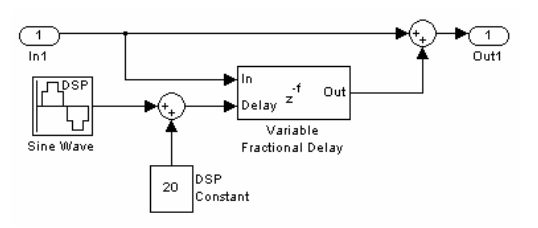
\includegraphics[width=\linewidth]{flanger.png}
    \caption{Simulink model of a flanger effect}
    \label{fig:flangersimulink}
\end{figure}

\subsubsection{Chorus}
The chorus effect was created with a simular phaser as the flanger. But instead of one phaser it uses four that are all one factor higher than the previous phaser. To a musician this sounds as a harmonic made of four flangers. 

\begin{figure}[ht]
    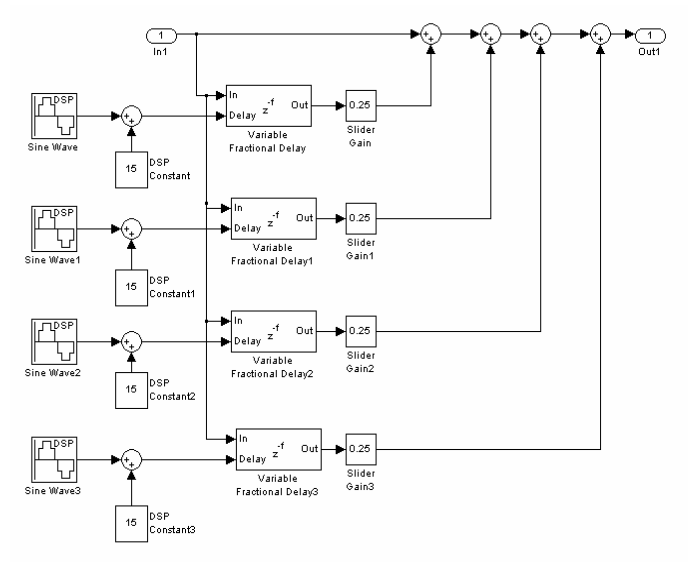
\includegraphics[width=\linewidth]{chorus.png}
    \caption{Simulink model of a chorus effect}
    \label{fig:chorussimulink}
\end{figure}

\subsubsection{Delay / echo}
The delay was the easiest of these effects to make. The delay adds a previously played delay to the original sound. 

\begin{figure}[ht]
    \includegraphics[width=\linewidth]{delay.png}
    \caption{Simulink model of a delay}
    \label{fig:delaysimulink}
\end{figure}

\newpage
